%! Author = Michelangelo Prisciano
%! Date = 30/11/2021

\documentclass{article}

% Language setting
% Replace `english' with e.g. `spanish' to change the document language
\usepackage[english]{babel}

% Set page size and margins
% Replace `letterpaper' with`a4paper' for UK/EU standard size
\usepackage[letterpaper,top=2cm,bottom=2cm,left=3cm,right=3cm,marginparwidth=1.75cm]{geometry}

% Useful packages
\usepackage{amsmath}
\usepackage{graphicx}
\usepackage[colorlinks=true, allcolors=blue]{hyperref}
\usepackage{tikz}
\usetikzlibrary{graphs,graphs.standard}

\title{Monte Carlo Simulation for Influence Models of Information Diffusion in Social Networks}
\author{Michelangelo Prisciano}

\begin{document}
\maketitle

\section{Introduction}

This project aims to follow up from the paper "Markov Chain Model Representation of Information Diffusion in Social Networks"
(\cite{monte_carlo_sim}) by exploring how information flows in a social network specifically with a threshold model.
This is based on the idea that an agent is most likely to adopt an idea when the number of its connection crosses a fixed threshold value.

\subsection{Keys and Objectives}
The goal of this project is to model the flow of information in a network through Markov Chains and a Monte Carlo simulation. The model adopted
initially is a combination of a threshold and probabilistic model, while other will be investigated at a later stage.

\section{Algorithm}
Starting with n infected seed nodes, we will follow how the infection progress through a combination of threshold and probabilistic
model. Every node that has a number of infected connections that crosses a set threshold will be infected with a probability p.
Suppose n is the total number of neighbour nodes of a particular node, k is the number of neighbour infected nodes. Then,
\[
    p = \frac{n-k}{n}
\]

In this scenario it is crucial to be able to access the number of infected connections of every node in a short amount of time,
preferably constant. An interesting way of keeping track of the number of infected connections of every node is through an array
of length n where n is the number of nodes in the graph. Initially the array is initialised in a way that every node has 0 infected
connections. As seed nodes are chosen and more nodes get infected, the array is updated in a "cascade" way. \newpage

For the sake of simplicity a pure threshold model is considered in this example. The complete graph \emph{g} has 6 nodes,
labelled from 0 to 5. Node 0 is chosen to be a seed infected node and the threshold \emph{t} is set to 1. \\ \\

\emph{Starting point}
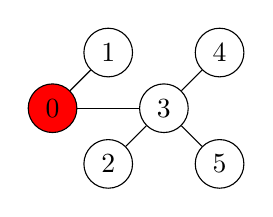
\begin{tikzpicture}[main/.style = {draw, circle}]
\node[main] (0) [fill=red]{$0$};
\node[main] (1) [above right of=0] {$1$};
\node[main] (2) [below right of=0] {$2$};
\node[main] (3) [above right of=2] {$3$};
\node[main] (4) [above right of=3] {$4$};
\node[main] (5) [below right of=3] {$5$};
\draw (0) -- (1);
\draw (0) -- (3);
\draw (3) -- (2);
\draw (3) -- (4);
\draw (3) -- (5);
\end{tikzpicture} \\

\begin{gather*}
[0\qquad1\qquad0\qquad1\qquad0\qquad0]\\
0\qquad1\qquad2\qquad3\qquad4\qquad5\\
\end{gather*}
Nodes 1 and 3 both have 1 infected connection, therefore \underline{the next nodes to be infected will be 1 and 3.} \\

\emph{Loop N1}
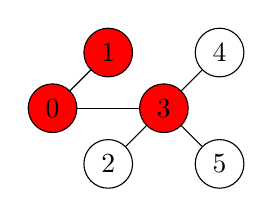
\begin{tikzpicture}[main/.style = {draw, circle}]
\node[main] (0) [fill=red]{$0$};
\node[main] (1) [above right of=0, fill=red] {$1$};
\node[main] (2) [below right of=0] {$2$};
\node[main] (3) [above right of=2, fill=red] {$3$};
\node[main] (4) [above right of=3] {$4$};
\node[main] (5) [below right of=3] {$5$};
\draw (0) -- (1);
\draw (0) -- (3);
\draw (3) -- (2);
\draw (3) -- (4);
\draw (3) -- (5);
\end{tikzpicture} \\

\begin{gather*}
    [2\qquad1\qquad1\qquad1\qquad1\qquad1]\\
    0\qquad1\qquad2\qquad3\qquad4\qquad5\\
\end{gather*}

Therefore, \underline{the next nodes to be infected will be 2, 4 and 5.} \\

\emph{Loop N2}
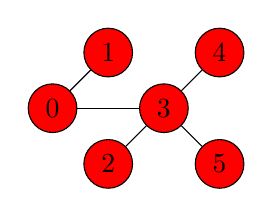
\begin{tikzpicture}[main/.style = {draw, circle}]
\node[main] (0) [fill=red]{$0$};
\node[main] (1) [above right of=0, fill=red] {$1$};
\node[main] (2) [below right of=0, fill=red] {$2$};
\node[main] (3) [above right of=2, fill=red] {$3$};
\node[main] (4) [above right of=3, fill=red] {$4$};
\node[main] (5) [below right of=3, fill=red] {$5$};
\draw (0) -- (1);
\draw (0) -- (3);
\draw (3) -- (2);
\draw (3) -- (4);
\draw (3) -- (5);
\end{tikzpicture} \\
\begin{gather*}
    [2\qquad1\qquad1\qquad4\qquad1\qquad1]\\
    0\qquad1\qquad2\qquad3\qquad4\qquad5\\
\end{gather*}

There are two more possible approaches to model the infection, merely a pure threshold and a pure probabilistic model. The former is
not that interesting due to the deterministic nature of the approach which is not versatile enough to model real world situations,
despite being a good starting point. The latter, on the other hand, is an approach which will be investigated at a later stage. The difference
is that there would be no threshold of infected connections to cross, every neighbour of an infected node will be infected with the probability
p mentioned earlier.
\section{Observations}

\bibliographystyle{alpha}
\bibliography{sample}

\end{document}